\pagestyle{fancy}
\section{Implementation}\label{sec:implementation}

The previous section defined the conceptual framework, the artifact's purpose as a research instrument, and the evaluation design that structures the comparative study. This section describes how those ideas were translated into a working system. The goal is not to document every engineering decision, but to make the technical design legible enough that the reader can assess whether the artifact faithfully operationalises the framework and whether the instrumentation is sufficient to support the evaluation.

\subsection{Architecture Overview}

The artifact is built as a full-stack web application using the Next.js App Router with TypeScript. The server layer exposes a set of API routes that handle participant management, trial orchestration, event logging, questionnaire storage, and ephemeral support generation. Persistent data is stored in a PostgreSQL database accessed through Drizzle~ORM, which provides type-safe queries and a migration-based schema workflow. The ephemeral support system relies on Google Gemini, accessed through the Vercel AI~SDK, to produce structured interface specifications from the current task state. The front end uses Tailwind~CSS and a component library based on Radix~UI primitives for consistent, accessible interface elements across both experimental conditions.

These choices reflect the requirements of a research instrument rather than a production application. Next.js was selected because its App Router collocates server-side logic and client rendering in the same project, which simplifies the instrumentation of both request handling and user interaction. TypeScript and Zod provide compile-time and runtime type safety across the generation pipeline, which is critical when validating AI-generated output against a constrained specification. PostgreSQL and Drizzle offer relational integrity and migration tooling appropriate for structured experimental data. The Vercel AI~SDK abstracts provider-specific details while supporting structured output modes, which allows the generation step to request JSON that conforms to a predefined schema rather than parsing free-form text.

\begin{figure}[htbp]
    \centering
    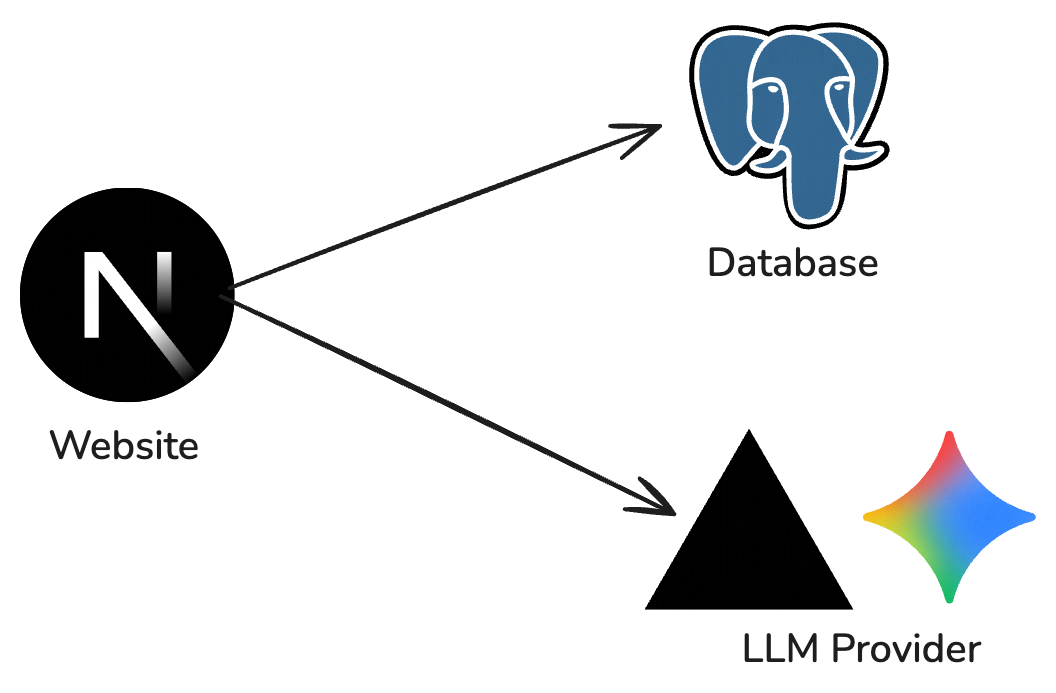
\includegraphics[width=0.95\textwidth]{graphics/architecture.png}
    \caption{High-level system architecture of the experimental artifact.}
    \label{fig:architecture}
\end{figure}

\subsection{Participant Flow and Session Management}

The study procedure described in the methodology is implemented as a linear state machine that determines which page the participant should see at any point during the session. When a participant first opens the website, they are presented with the study information and consent form. Providing consent creates a participant record in the database and sets an HTTP-only session cookie that associates all subsequent requests with that record. No traditional authentication is required because the study collects no directly identifying personal data; the cookie serves only to link a browser session to its corresponding participant row.

After consenting, the participant completes a short background questionnaire covering age range, occupation, familiarity with web applications, and familiarity with AI-assisted tools. Submitting the background questionnaire acknowledges the study instructions and triggers the creation of the first trial row. From this point forward, a server-side state resolution function inspects the participant's record, their trial rows, and their questionnaire responses to determine the current study step. The possible steps form a fixed sequence: \emph{background}, \emph{study} (an active trial), \emph{post-trial questionnaire}, \emph{final questionnaire}, and \emph{complete}. The client-side routing function maps each step to the corresponding page, so that refreshing the browser or navigating away always returns the participant to the correct point in the procedure.

Trial rows are created incrementally rather than all at once. The first trial is created when the participant acknowledges the instructions. Each subsequent trial is created only after the previous trial has been completed and its post-trial questionnaire has been submitted. This ensures that the participant cannot skip ahead or access later trials before finishing earlier ones.

Counterbalancing is implemented at the participant level. When a participant record is created, a boolean flag is randomly set to determine whether the baseline condition corresponds to Version~A or Version~B. The trial plan then assigns conditions to version labels using this flag, so that one participant may encounter the baseline first while another encounters the ephemeral condition first, both under the neutral label ``Version~A.'' The content variant for each condition is further diversified by hashing the participant identifier together with the scenario identifier, ensuring that the specific slide deck a participant sees in the baseline condition differs from the one they see in the ephemeral condition.

\subsection{Data Model}

The database schema consists of five tables designed to capture the behavioural and self-reported data required by the evaluation measures defined in the methodology. Figure~\ref{fig:data-model-erd} shows the entity--relationship structure: each participant may complete several trials; each trial may emit many logged events and many stored ephemeral support generations; questionnaire responses belong to a participant, and may optionally reference a trial (post-trial items) or omit a trial key (final questionnaire). Table~\ref{tab:schema} summarises what each table contributes to the evaluation. The \texttt{trial\_events} table also stores \texttt{participant\_id} for efficient querying, in addition to \texttt{trial\_id}; the diagram omits that redundant edge for clarity.

\begin{figure}[htbp]
    \centering
    \resizebox{0.95\textwidth}{!}{%
    \begin{tikzpicture}[
        font=\small,
        ent/.style={
            draw,
            rounded corners,
            align=center,
            inner sep=7pt,
            minimum width=2.6cm,
            minimum height=1.05cm
        },
        card/.style={font=\scriptsize, inner sep=1pt}
    ]
    \node[ent] (P) {participants};
    \node[ent, below=1.35cm of P] (T) {trials};
    \node[ent, below left=1.05cm and 0.15cm of T] (E) {trial\_events};
    \node[ent, below right=1.05cm and 0.15cm of T] (S) {support\_outputs};
    \node[ent, right=3.1cm of T] (Q) {questionnaire\_responses};

    \draw[->, semithick] (P) -- node[card, right] {1:N} (T);
    \draw[->, semithick] (T) -- node[card, left, xshift=-1mm] {1:N} (E);
    \draw[->, semithick] (T) -- node[card, right, xshift=1mm] {1:N} (S);
    \draw[->, semithick] (P.east) to[out=8, in=160] node[card, above, sloped, near start] {1:N} (Q.west);
    \draw[->, semithick, dashed] (T.east) -- node[card, below, midway] {1:N\textsuperscript{*}} (Q.west);
    \end{tikzpicture}%
    }
    \caption{Entity--relationship diagram of the study database. Directed edges are labelled with cardinalities: one participant to many trials; one trial to many events and many support records; one participant to many questionnaire rows. The dashed edge indicates an optional foreign key: \texttt{trial\_id} is \texttt{NULL} for final-questionnaire rows.}
    \label{fig:data-model-erd}
\end{figure}

\begin{table}[htbp]
    \centering
    \small
    \caption{Summary of each table's role relative to the evaluation measures. Full column definitions follow the Drizzle schema in the artifact.}
    \label{tab:schema}
    \begin{tabular}{@{}p{0.28\textwidth}p{0.62\textwidth}@{}}
        \toprule
        Table & Role in the study \\
        \midrule
        \texttt{participants} & Consent and background questionnaire; counterbalancing flag (\texttt{baseline\_is\_version\_a}); links all rows for a session. \\
        \texttt{trials} & One row per task trial: condition, scenario, timing, correctness, submitted answer, interaction count---supports performance and efficiency measures. \\
        \texttt{trial\_events} & Typed events with JSON payloads---supports interaction counts and ephemeral engagement (e.g.\ support shown, dismissed). \\
        \texttt{questionnaire\_responses} & Post-trial Likert items and final preference; \texttt{trial\_id} set for post-trial rows, null for final rows---supports subjective measures. \\
        \texttt{support\_outputs} & Ephemeral condition only: model input state and output spec per generation---supports analysis of support quality and fallback. \\
        \bottomrule
    \end{tabular}
\end{table}

Foreign key constraints with cascading deletion ensure referential integrity: deleting a participant removes all associated trials, events, questionnaire responses, and support outputs. Indexes on participant identifiers, trial identifiers, and event types support efficient querying during data export and analysis.

\subsection{Task Scenario Implementation}

The study evaluates one scenario, the slide-reordering task described in the methodology, under two experimental conditions. The implementation uses a scenario registry that defines each scenario's metadata, including its taxonomy category, correct answer, allowed ephemeral targets, task prompts, and a function that builds the initial task state. This registry-based design means that adding a new scenario requires only a new registry entry rather than changes to the study flow or state machine.

The slide-reordering scenario presents participants with a short deck of four slides whose order has been intentionally scrambled. The main canvas area displays a read-only preview of the currently selected slide, while the actual task interaction occurs through a horizontal strip of draggable thumbnail cards. Drag-and-drop is implemented using the \texttt{@dnd-kit} library, which provides accessible keyboard and pointer-based reordering with sortable constraints. Participants reorder the strip and submit when they believe the sequence is correct.

Correctness is evaluated by comparing the submitted slide order against a predefined canonical order. Each scenario variant defines its own canonical sequence: variant~A follows a corporate readout structure (title, problem, metrics, ask), while variant~B follows a committee funding structure (meeting frame, policy, proof, ballot items). The variant assignment uses a deterministic hash of the participant identifier and scenario identifier to assign variant~A or variant~B to the baseline condition, with the opposite variant assigned to the ephemeral condition. This ensures that each participant encounters two different slide decks across the two trials, preventing familiarity effects from the task content while keeping the task structure identical.

Both conditions share the same task component, the same interaction mechanics, and the same submission logic. The only difference is whether the ephemeral support layer is active, which is controlled by the condition field on the trial row. This design isolates the effect of ephemeral augmentation from other variables.

\subsection{Ephemeral Support System}

The ephemeral support system is the core technical contribution of the artifact. It translates the framework's concepts of taxonomy, lifecycle, and design principles into a constrained generative pipeline that produces temporary interface overlays without replacing the host application. This subsection describes the three layers of the system: the specification model that defines what can be generated, the pipeline that produces and validates specifications, and the rendering layer that displays them.

\subsubsection{Component Specification Model}

Ephemeral support is represented as a typed tree structure called an \texttt{EphemeralSpec}. Each specification contains a version number, a root node, and metadata indicating whether the overlay is dismissible. Nodes are recursive: each node has a type, a property bag validated against a per-type schema, and optional children. The tree is constrained to a maximum depth of four levels and a maximum of six children per node.

The component catalog defines seventeen component types, organised into five functional categories. Table~\ref{tab:component-catalog} lists the types and their roles. Visual cue components draw attention to specific interface elements without adding content. Anchored annotation components attach textual or rich content near a target element. Relational components connect or compare two or more targets to support reasoning across elements. Layout containers position children within the viewport or relative to a target. Rich content components render sanitised HTML and inline SVG for more expressive explanations such as flow diagrams or annotated illustrations.

\begin{table}[htbp]
    \centering
    \small
    \caption{Ephemeral component catalog (version~3). Each type is validated against a per-component Zod schema that enforces field types, string lengths, and structural constraints.}
    \label{tab:component-catalog}
    \begin{tabular}{@{}p{0.22\textwidth}p{0.26\textwidth}p{0.44\textwidth}@{}}
        \toprule
        Category & Component type & Role \\
        \midrule
        Visual cues & \texttt{HighlightRing} & Amber ring around a target element \\
        & \texttt{PulseRing} & Animated ring with configurable duration \\
        & \texttt{ArrowCue} & Arrow pointing at a target \\
        & \texttt{FocusMask} & Dims everything except the target \\
        \midrule
        Anchored annotations & \texttt{AnchoredTooltip} & Plain-text tooltip near a target \\
        & \texttt{HintStack} & Ordered list of short hints near a target \\
        & \texttt{InspectPanel} & Expandable panel with summary and optional detail lines \\
        & \texttt{ConsequenceNote} & Single italic consequence line near a target \\
        & \texttt{SideNote} & Margin annotation beside a target \\
        \midrule
        Relational & \texttt{ConnectorLine} & Dashed line between two targets \\
        & \texttt{ComparisonStrip} & Short contrast text positioned under two targets \\
        & \texttt{StepRail} & Numbered callouts across two to six targets \\
        \midrule
        Layout containers & \texttt{Stack} & Vertical sequence container \\
        & \texttt{ViewportPanel} & Absolutely positioned panel in viewport percentages \\
        & \texttt{TargetOffsetPanel} & Panel positioned relative to a target with pixel offsets \\
        \midrule
        Rich content & \texttt{FlowHtml} & Sanitised HTML block (only inside \texttt{ViewportPanel}) \\
        & \texttt{AnchoredHtml} & Sanitised HTML anchored near a target \\
        \bottomrule
    \end{tabular}
\end{table}

Each component type is associated with a Zod schema that validates its properties at runtime. These schemas enforce constraints such as maximum string lengths, numeric ranges, and required fields. For example, an \texttt{InspectPanel} requires a target identifier, a title of at most 120~characters, a summary of at most 280~characters, and optionally up to four detail lines of at most 200~characters each. These limits prevent the model from generating excessively long or unbounded output while leaving enough room for contextually relevant content.

The catalog is versioned so that changes to the available component types or their constraints can be tracked across study sessions. The current study uses catalog version~3.

\subsubsection{Generation and Validation Pipeline}\label{sec:pipeline}

When ephemeral support is requested during a trial, the system executes a multi-stage pipeline that generates a specification, validates it against the catalog and scenario constraints, and either accepts it or falls back to a deterministic alternative. Figure~\ref{fig:ephemeral-pipeline-impl} illustrates this pipeline.

The generation step constructs two prompts. The system prompt describes the specification schema, lists all available component types with their property schemas, states the allowed target identifiers for the current scenario, provides taxonomy-specific guidance (such as which components are most appropriate for refinement support), and enumerates the design rules that constrain output structure. The user prompt includes the current task state, including slide order, deck metadata, and review goals, together with an optional participant interaction snapshot that reflects the participant's progress at the moment support was requested. This snapshot allows the model to tailor its output to what the participant has already done rather than generating generic first-visit guidance.

The system sends these prompts to Google Gemini using the Vercel AI~SDK's structured output mode, which constrains the model to produce JSON conforming to a provided Zod schema. The schema used for model output is a simplified subset of the full specification schema, designed to avoid compatibility issues with the provider's structured output implementation while remaining strict enough to prevent most structural errors at generation time.

The model's output then passes through a series of server-side validation stages:

\begin{enumerate}
    \item \textbf{Envelope parsing.} The top-level structure is checked for a valid version number, root node, and metadata.
    \item \textbf{Node tree parsing.} The root and its descendants are recursively validated for correct node shape, child count limits, and maximum depth.
    \item \textbf{Per-component property validation.} Each node's properties are validated against its type-specific Zod schema, enforcing field types, string lengths, and numeric ranges.
    \item \textbf{Target allowlisting.} Every target identifier referenced in the specification is checked against the scenario's predefined list of allowed targets. Any reference to an interface element not declared in the scenario registry causes the specification to be rejected.
    \item \textbf{Structural container rules.} Layout containers are checked to ensure they contain at least one child. This applies to \texttt{Stack}, \texttt{ViewportPanel}, and \texttt{TargetOffsetPanel}.
    \item \textbf{Ancestry constraints.} \texttt{FlowHtml} nodes are permitted only within a \texttt{ViewportPanel} subtree, preventing free-floating rich HTML from appearing anywhere in the interface.
    \item \textbf{HTML sanitisation.} Any HTML content in \texttt{FlowHtml}, \texttt{AnchoredHtml}, or \texttt{SideNote} nodes is passed through a server-side sanitisation step using DOMPurify with a strict allowlist of tags and attributes. This prevents injection of scripts, event handlers, or disallowed elements while permitting semantic HTML and inline SVG for diagrams.
\end{enumerate}

If any stage rejects the output, the system falls back to a deterministic, hardcoded specification for the current scenario. Fallback specifications are defined per scenario and per variant, ensuring that every participant in the ephemeral condition receives some form of support regardless of model behaviour. The fallback specifications use the same component types and target identifiers as model-generated output, so they appear visually consistent with the rest of the ephemeral experience.

Whether the specification was model-generated or a fallback, the full input state, model name, and output are persisted to the \texttt{support\_outputs} table. This logging enables post-study analysis of generation quality, fallback frequency, and the relationship between input context and output content.

To verify this implementation end-to-end outside the aggregate study analysis, the pipeline was also tested locally against the real \texttt{/api/support} route on 2026-04-04. Three consecutive hesitation-triggered requests for the \texttt{slides-outline-refine} scenario completed successfully and were persisted as \texttt{support\_outputs} rows 101--103, all with \texttt{usedFallback = false} and \texttt{modelName = gemini-2.0-flash}. The richest of these records (row 103) produced a \texttt{Stack}-rooted specification containing \texttt{StepRail}, \texttt{InspectPanel}, \texttt{ConnectorLine}, and \texttt{AnchoredTooltip} nodes, demonstrating that a non-trivial multi-component overlay could be generated, validated, saved to PostgreSQL, and rendered without falling back. A condensed excerpt of this local trace is included in Appendix~\ref{app:local-generation-trace}.

\begin{figure}[htbp]
    \centering
    \resizebox{0.98\textwidth}{!}{%
    \begin{tikzpicture}[
        font=\footnotesize,
        node distance=7mm and 7mm,
        box/.style={
            draw,
            rounded corners,
            align=left,
            inner sep=6pt,
            text width=4.2cm
        },
        wide/.style={
            draw,
            rounded corners,
            align=left,
            inner sep=6pt,
            text width=5.7cm
        },
        small/.style={
            draw,
            rounded corners,
            align=left,
            inner sep=6pt,
            text width=3.9cm
        }
    ]
    \node[box] (trigger) {\textbf{1. Client trigger}\\
    In \texttt{app/study/page.tsx}, support is triggered after hesitation or by explicit request. The client sends \texttt{participantId}, \texttt{trialId}, \texttt{scenarioId}, trigger reason, and an optional participant snapshot to \texttt{POST /api/support}.};

    \node[box, right=of trigger] (route) {\textbf{2. Route checks and state assembly}\\
    \texttt{app/api/support/route.ts} verifies the session cookie, trial ownership, scenario match, and that the active condition is ephemeral. It reconstructs the baseline task state and validates the participant snapshot for the scenario.};

    \node[box, right=of route] (prompt) {\textbf{3. Prompt construction and model call}\\
    \texttt{generateValidatedSupport()} builds the system prompt from the component catalog, allowed target IDs, and taxonomy guidance, then combines it with task state and participant progress before calling Gemini through the Vercel AI SDK.};

    \node[wide, below=of route] (validate) {\textbf{4. Spec parsing and validation}\\
    Model output is coerced into the app envelope and checked in order for: (1) envelope parsing, (2) node-tree parsing, (3) per-component Zod prop validation, (4) target allowlisting, (5) structural container rules, (6) \texttt{FlowHtml} ancestry constraints, and (7) HTML sanitisation.};

    \node[small, below left=of validate] (accept) {\textbf{5a. Accept model spec}\\
    A valid \texttt{EphemeralSpec} becomes the support payload together with the discovered component types and catalog version.};

    \node[small, below right=of validate] (fallback) {\textbf{5b. Deterministic fallback}\\
    Missing API key, empty structured output, parse failure, rule violation, or SDK error causes \texttt{buildFallbackSpec()} to return a scenario-specific backup spec.};

    \node[wide, below=11mm of validate] (persist) {\textbf{6. Persist generation record}\\
    The route inserts a row into \texttt{support\_outputs} containing the input state (baseline task state, participant snapshot, trigger) and the output bundle (catalog version, final spec, component types, trigger, and whether fallback was used).};

    \node[wide, below=of persist] (render) {\textbf{7. Return JSON and render overlay}\\
    The API returns \texttt{spec} plus metadata to the study page. The client sets local state, \texttt{EphemeralLayer} renders the overlay above the existing interface, and later dismiss/use/inspect interactions are logged separately.};

    \draw[->, semithick] (trigger) -- (route);
    \draw[->, semithick] (route) -- (prompt);
    \draw[->, semithick] (prompt) -- (validate);
    \draw[->, semithick] (validate) -- (accept);
    \draw[->, semithick] (validate) -- (fallback);
    \draw[->, semithick] (accept) -- (persist);
    \draw[->, semithick] (fallback) -- (persist);
    \draw[->, semithick] (persist) -- (render);
    \end{tikzpicture}%
    }
    \caption{Ephemeral support generation and validation pipeline. Model output passes through seven validation stages before rendering; invalid output triggers a deterministic fallback. Both paths are logged for later analysis.}
    \label{fig:ephemeral-pipeline-impl}
\end{figure}

\subsubsection{Rendering Layer}

Accepted specifications are rendered as a temporary overlay above the existing application interface using a React portal. The overlay component receives the validated specification tree and recursively dispatches each node to its corresponding catalog component based on the node's type. This dispatch model means that the renderer does not need to know about the content of any particular specification; it only needs to map types to components and pass through validated properties.

Components that reference target elements, such as \texttt{HighlightRing}, \texttt{AnchoredTooltip}, or \texttt{ConnectorLine}, resolve their targets by looking up DOM elements by identifier. A custom hook observes the target element's bounding rectangle and updates the overlay position when the layout changes, for example when the browser is resized or when other elements shift. A viewport clamping utility ensures that anchored components remain visible even when their target is near the edge of the screen.

The overlay respects the lifecycle stage of dismissal defined in the framework. When the specification's metadata marks the overlay as dismissible, a close control is rendered that allows the participant to remove the support at any time. Dismissal fires a logged event so that the analysis can distinguish between support that was actively used and support that was dismissed without engagement. The overlay does not persist across page navigations or trial boundaries, which enforces the ephemerality principle at the session level.

\subsection{Instrumentation and Logging}

The evaluation design in the methodology specifies several behavioural and self-reported measures. The artifact implements a corresponding instrumentation layer that captures the data needed for each measure.

Client-side interaction events are sent to a logging API endpoint that inserts rows into the \texttt{trial\_events} table. Each event includes a type label and a JSON payload with contextual details. A predefined set of event types is recognised as countable interactions, and the trial's running interaction count is incremented automatically when one of these events is recorded. Table~\ref{tab:event-types} lists the event types and their relationship to the evaluation measures.

\begin{table}[htbp]
    \centering
    \small
    \caption{Logged event types and their relationship to evaluation measures. Events marked with an asterisk (*) increment the trial's interaction count.}
    \label{tab:event-types}
    \begin{tabular}{@{}p{0.33\textwidth}p{0.41\textwidth}p{0.18\textwidth}@{}}
        \toprule
        Event type & When recorded & Evaluation measure \\
        \midrule
        \texttt{trial\_viewed}* & Participant opens a trial & Interaction count \\
        \texttt{slide\_reordered}* & A slide is dragged to a new position & Interaction count \\
        \texttt{answer\_selected}* & An answer is first chosen & Interaction count \\
        \texttt{answer\_changed}* & An answer is revised & Interaction count \\
        \midrule
        \texttt{support\_requested}* & Participant explicitly requests support & Support engagement \\
        \texttt{support\_triggered}* & Support is triggered automatically & Support engagement \\
        \texttt{support\_shown}* & Support overlay becomes visible & Support engagement \\
        \texttt{support\_dismissed}* & Participant closes the overlay & Support engagement \\
        \texttt{support\_used}* & Participant acts on the support & Support engagement \\
        \texttt{support\_ignored}* & Support is present but not interacted with & Support engagement \\
        \texttt{support\_inspect\_expanded}* & Participant expands an \texttt{InspectPanel} detail section & Support engagement \\
        \bottomrule
    \end{tabular}
\end{table}

For the ephemeral condition, additional data is captured beyond interaction events. Each call to the support generation endpoint persists the full input state (task state and participant snapshot), the model name, and the complete output specification to the \texttt{support\_outputs} table. This allows the analysis to examine not only whether support was shown and used, but also what the system produced and why, including whether a fallback was triggered.

Questionnaire responses are stored as individual question--response pairs rather than as monolithic form submissions. Post-trial ratings for intrusiveness, perceived control, and helpfulness are linked to the specific trial they follow, while final comparative questions are linked only to the participant. This structure supports direct joins between behavioural data and subjective ratings at the trial level.

A data export endpoint produces a structured bundle of all study data, protected by a server-side secret. The export includes participant records, trial summaries with performance metrics, event logs, questionnaire responses, and support generation outputs, providing the complete dataset needed for the analysis plan described in the methodology.
